% Architecture schematic of the current surrogate (sim2reco.models.surrogate.Surrogate, tier2=True).
% Compile: bash scripts/render_schematic.sh. Update this file when the architecture changes.
\documentclass[tikz,border=6pt]{standalone}
\usetikzlibrary{positioning,fit,arrows.meta,calc,backgrounds}
\usepackage[T1]{fontenc}
\usepackage{amsmath,amssymb}
\usepackage{helvet}\renewcommand{\familydefault}{\sfdefault}
\definecolor{ink}{HTML}{222222}
\definecolor{paper}{HTML}{FFFFFF}
\definecolor{cin}{HTML}{0072B2}    % inputs
\definecolor{cenc}{HTML}{009E73}   % encoder
\definecolor{ccls}{HTML}{D55E00}   % classification heads
\definecolor{cgen}{HTML}{E69F00}   % generative heads
\definecolor{cout}{HTML}{555555}   % decoder / output
\tikzset{
  box/.style={draw=ink, line width=1.2pt, rounded corners=3pt, fill=paper, align=left, inner sep=6pt, font=\small, text=ink},
  head/.style={box, text width=84mm},
  stage/.style={font=\footnotesize\bfseries, text=ink!80, anchor=south west},
  dim/.style={font=\scriptsize, text=ink!70},
  arr/.style={-{Latex[length=2.2mm]}, line width=0.7pt, draw=ink},
  arrd/.style={arr, dashed},
  arrc/.style={arr, dotted, line width=0.9pt},
}
\begin{document}
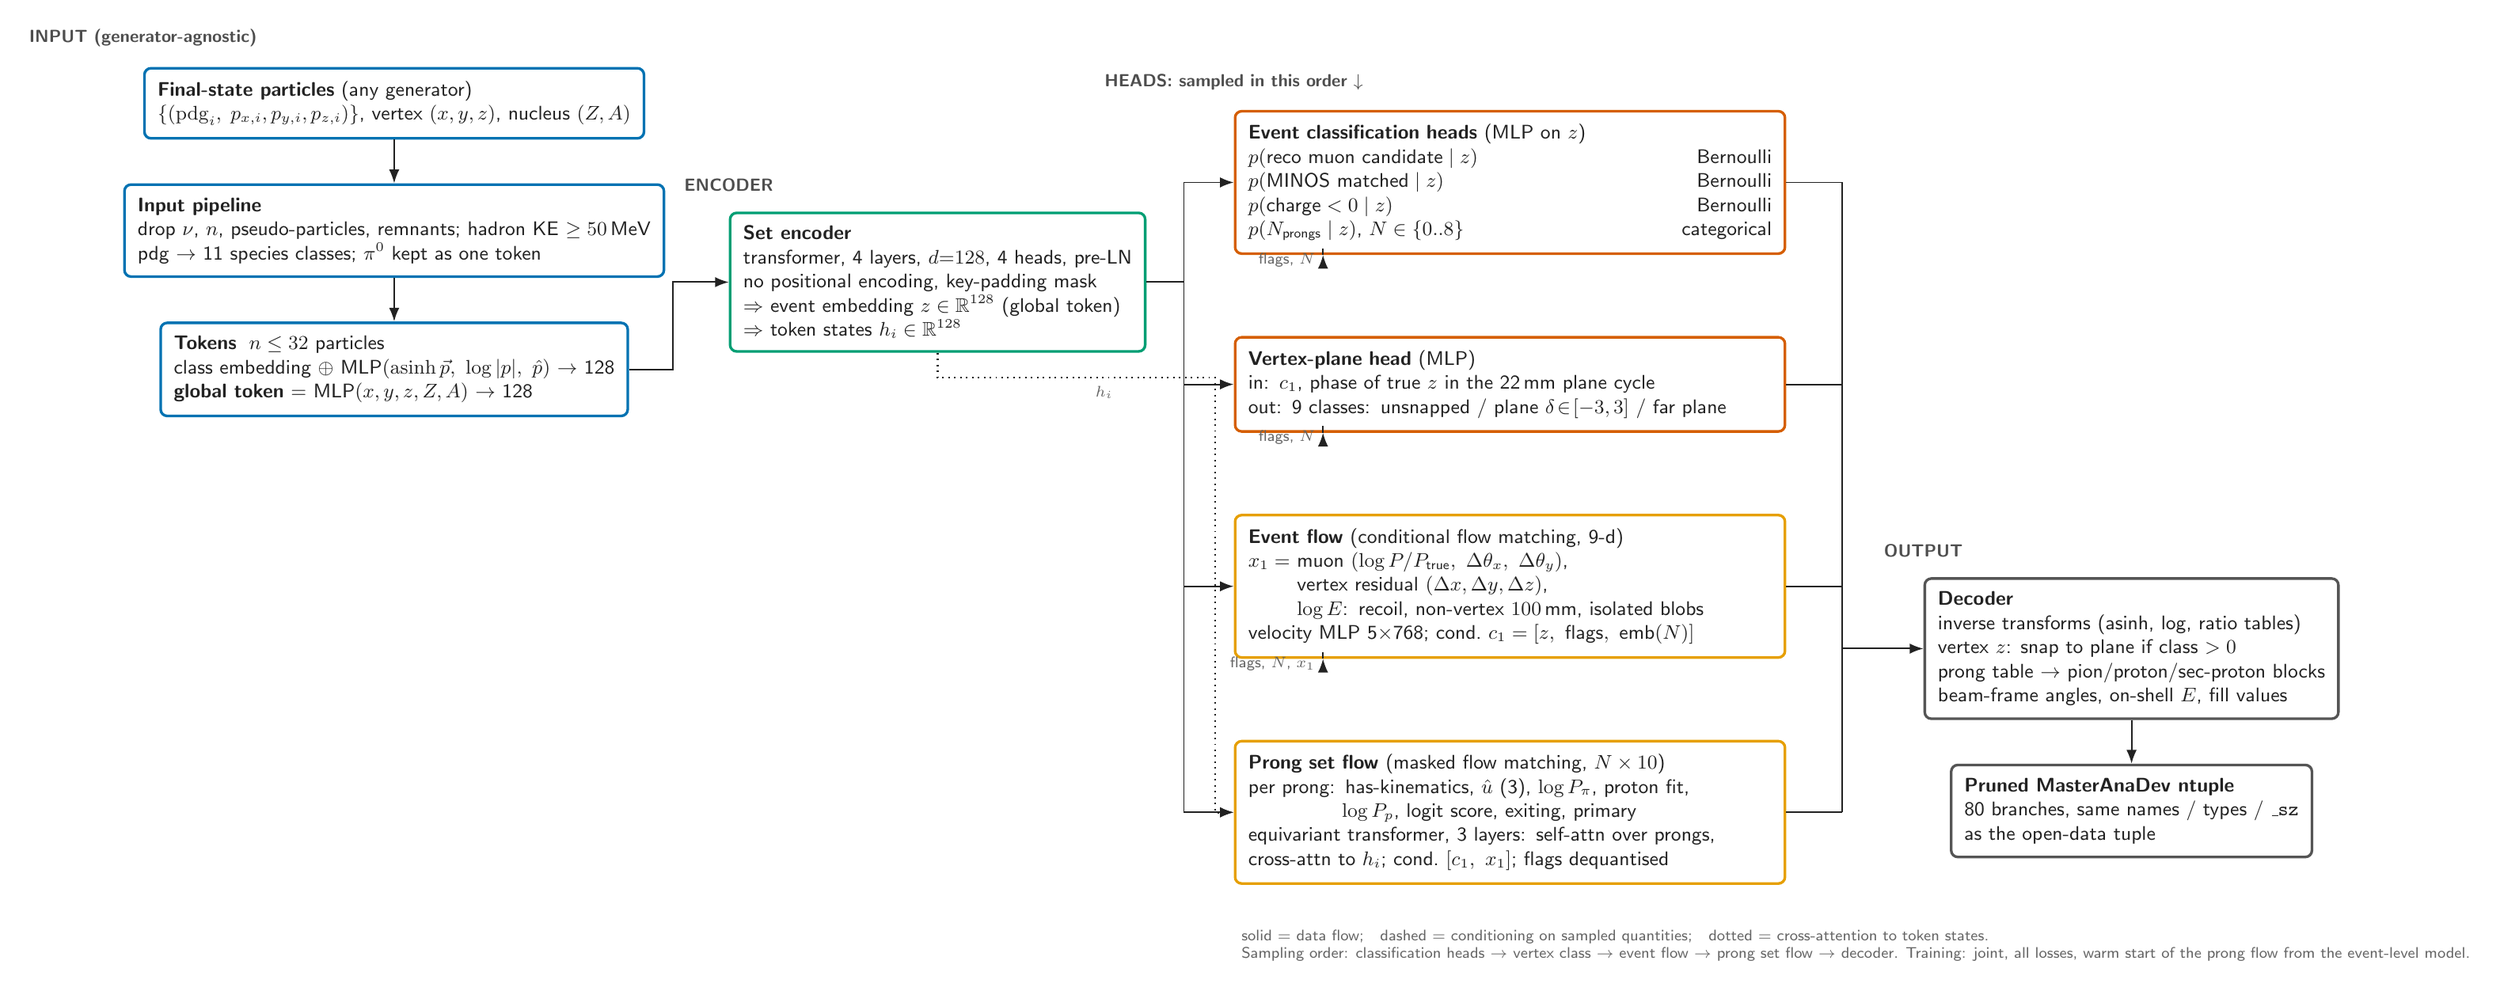
\begin{tikzpicture}[node distance=7mm and 9mm]

% ---------------- inputs ----------------
\node[box, draw=cin] (gen) {\textbf{Final-state particles} (any generator)\\
  $\{(\mathrm{pdg}_i,\;p_{x,i},p_{y,i},p_{z,i})\}$, vertex $(x,y,z)$, nucleus $(Z,A)$};
\node[box, draw=cin, below=of gen] (pipe) {\textbf{Input pipeline}\\
  drop $\nu$, $n$, pseudo-particles, remnants; hadron KE $\ge 50$\,MeV\\
  pdg $\to$ 11 species classes; $\pi^0$ kept as one token};
\node[box, draw=cin, below=of pipe] (tok) {\textbf{Tokens} $\;n \le 32$ particles\\
  class embedding $\oplus$ MLP$(\mathrm{asinh}\,\vec p,\ \log|p|,\ \hat p)$ $\to$ 128\\
  \textbf{global token} $=$ MLP$(x,y,z,Z,A)$ $\to$ 128};

% ---------------- encoder ----------------
\node[box, draw=cenc, right=16mm of tok.east, anchor=west, yshift=14mm] (enc) {\textbf{Set encoder}\\
  transformer, 4 layers, $d{=}128$, 4 heads, pre-LN\\
  no positional encoding, key-padding mask\\
  $\Rightarrow$ event embedding $z\in\mathbb{R}^{128}$ (global token)\\
  $\Rightarrow$ token states $h_i\in\mathbb{R}^{128}$};

% ---------------- classification heads ----------------
\node[head, draw=ccls, right=14mm of enc.east, anchor=west, yshift=16mm] (t0) {\textbf{Event classification heads} (MLP on $z$)\\
  $p(\text{reco muon candidate}\mid z)$ \hfill Bernoulli\\
  $p(\text{MINOS matched}\mid z)$ \hfill Bernoulli\\
  $p(\text{charge}<0\mid z)$ \hfill Bernoulli\\
  $p(N_\text{prongs}\mid z)$, $N\in\{0..8\}$ \hfill categorical};
\node[head, draw=ccls, below=13mm of t0.south west, anchor=north west] (vtx) {\textbf{Vertex-plane head} (MLP)\\
  in: $c_1$, phase of true $z$ in the 22\,mm plane cycle\\
  out: 9 classes: unsnapped / plane $\delta\!\in\![-3,3]$ / far plane};

% ---------------- generative heads ----------------
\node[head, draw=cgen, below=13mm of vtx.south west, anchor=north west] (t1) {\textbf{Event flow} (conditional flow matching, 9-d)\\
  $x_1 = $ muon $(\log P/P_\text{true},\ \Delta\theta_x,\ \Delta\theta_y)$,\\
  \hphantom{$x_1 = $} vertex residual $(\Delta x,\Delta y,\Delta z)$,\\
  \hphantom{$x_1 = $} $\log E$: recoil, non-vertex $100$\,mm, isolated blobs\\
  velocity MLP 5$\times$768; cond.\ $c_1=[z,\ \text{flags},\ \text{emb}(N)]$};
\node[head, draw=cgen, below=13mm of t1.south west, anchor=north west] (t2) {\textbf{Prong set flow} (masked flow matching, $N\times 10$)\\
  per prong: has-kinematics, $\hat u$ (3), $\log P_\pi$, proton fit,\\
  \hphantom{per prong:} $\log P_p$, logit score, exiting, primary\\
  equivariant transformer, 3 layers: self-attn over prongs,\\
  cross-attn to $h_i$; cond.\ $[c_1,\ x_1]$; flags dequantised};

% ---------------- decoder / output ----------------
\node[box, draw=cout, right=22mm of t1.east, anchor=west, yshift=-10mm] (dec) {\textbf{Decoder}\\
  inverse transforms (asinh, log, ratio tables)\\
  vertex $z$: snap to plane if class $>0$\\
  prong table $\to$ pion/proton/sec-proton blocks\\
  beam-frame angles, on-shell $E$, fill values};
\node[box, draw=cout, below=of dec] (nt) {\textbf{Pruned MasterAnaDev ntuple}\\
  80 branches, same names / types / \texttt{\_sz}\\
  as the open-data tuple};

% ---------------- arrows ----------------
\draw[arr] (gen) -- (pipe);
\draw[arr] (pipe) -- (tok);
\draw[arr] (tok.east) -- ++(7mm,0) |- (enc.west);
\draw[arr] (enc.east) -- ++(6mm,0) |- (t0.west);
\draw[arr] (enc.east) -- ++(6mm,0) |- (vtx.west);
\draw[arr] (enc.east) -- ++(6mm,0) |- (t1.west);
\draw[arr] (enc.east) -- ++(6mm,0) |- (t2.west);
\draw[arrc] (enc.south) -- ++(0,-4mm) -| ($(t2.west)+(-3mm,0)$) node[dim, pos=0.3, below] {$h_i$} -- (t2.west);
% conditioning on sampled quantities (dashed, inside the head column)
\draw[arrd] ($(t0.south)+(-30mm,0)$) -- ($(t0.south)+(-30mm,0)$ |- vtx.north) node[dim, pos=0.5, left, yshift=-0.8mm] {flags, $N$};
\draw[arrd] ($(vtx.south)+(-30mm,0)$) -- ($(vtx.south)+(-30mm,0)$ |- t1.north) node[dim, pos=0.5, left, yshift=-0.8mm] {flags, $N$};
\draw[arrd] ($(t1.south)+(-30mm,0)$) -- ($(t1.south)+(-30mm,0)$ |- t2.north) node[dim, pos=0.5, left, yshift=-0.8mm] {flags, $N$, $x_1$};
% outputs collected on a bus to the decoder
\coordinate (bus) at ($(t0.east)+(9mm,0)$);
\foreach \h in {t0,vtx,t1,t2} { \draw[line width=0.7pt, draw=ink] (\h.east) -- (\h.east -| bus); }
\draw[line width=0.7pt, draw=ink] (t0.east -| bus) -- (t2.east -| bus);
\draw[arr] (dec.west -| bus) -- (dec.west);
\draw[arr] (dec) -- (nt);

% ---------------- stage labels ----------------
\node[stage, above=2mm of gen.north west] {INPUT (generator-agnostic)};
\node[stage, above=2mm of enc.north west] {ENCODER};
\node[stage, above=2mm of t0.north west] {HEADS: sampled in this order $\downarrow$};
\node[stage, above=2mm of dec.north west, xshift=0mm] {OUTPUT};

% ---------------- legend ----------------
\node[dim, below=6mm of t2.south west, anchor=north west, align=left] {
  solid $=$ data flow;\quad dashed $=$ conditioning on sampled quantities;\quad dotted $=$ cross-attention to token states.\\
  Sampling order: classification heads $\to$ vertex class $\to$ event flow $\to$ prong set flow $\to$ decoder.
  Training: joint, all losses, warm start of the prong flow from the event-level model.};

\end{tikzpicture}
\end{document}
